
%\documentclass[conference]{IEEEtran}


\documentclass[a4paper]{llncs}



\usepackage{a4wide}
\usepackage{graphicx}
\usepackage[vlined,ruled]{algorithm2e}
\usepackage{xcolor}
\usepackage{listings}
\usepackage{listings-golang}
\usepackage{hyperref}
\usepackage{subcaption}


\definecolor{lightgray}{rgb}{.9,.9,.9}
\definecolor{darkgray}{rgb}{.4,.4,.4}
\definecolor{purple}{rgb}{0.65, 0.12, 0.82}
\definecolor{mygray}{rgb}{0.5,0.5,0.5}
\definecolor{mygreen}{rgb}{0,0.6,0}

\hypersetup{
    colorlinks,
    linkcolor={red},
    citecolor={blue},
    urlcolor={blue}
}

\lstset{ % add your own preferences
    basicstyle=\footnotesize,
    keywordstyle=\color{red},
    numbers=left,
    numbersep=5pt,
    showstringspaces=false, 
    stringstyle=\color{blue},
    tabsize=4,
    language=Golang % this is it !
}




\begin{document}
%
% paper title
% can use linebreaks \\ within to get better formatting as desired
\title{Inferring Invariants of Distributed Programs}


% author names and affiliations
% use a multiple column layout for up to three different
% affiliations

\author{Arash Vahabzadeh \and Keheliya Gallaba}
\institute{University of British Columbia,\\
Vancouver, Canada\\
\mailsa}

\urldef{\mailsa}\path|{arashvhb,kgallaba}@ece.ubc.ca| 

% \author{\IEEEauthorblockN{Keheliya Gallaba\IEEEauthorrefmark{1},
% Arash Vahabzadeh\IEEEauthorrefmark{2}}
% \IEEEauthorblockA{University of British Columbia\\
% Vancouver, BC, Canada\\
% Email: \IEEEauthorrefmark{1}kgallaba@ece.ubc.ca,
% \IEEEauthorrefmark{2}arashvhb@ece.ubc.ca}}






% make the title area
\maketitle




% For peer review papers, you can put extra information on the cover
% page as needed:
% \ifCLASSOPTIONpeerreview
% \begin{center} \bfseries EDICS Category: 3-BBND \end{center}
% \fi
%
% For peerreview papers, this IEEEtran command inserts a page break and
% creates the second title. It will be ignored for other modes.
%\IEEEpeerreviewmaketitle



\section{Abstract}
\section{Introduction}

Building a reliable distributed system is a difficult task, since distributed system should continue operating even when components or the network fail, this means that there are many corner cases that developers should consider when building a system. Building such 
a reliable and dependable system is not possible without thorough testing. However, testing a distributed system is a difficult task because it is hard to test components of a distributed system in isolation. There are many 
failure scenarios that a distributed system should handle and these scenarios should be tested as well. In some cases reproducing the failures is a difficult task e.g., degrading network performance for test purposes. Many bugs turn out to be heisenbugs in a distributed 
system which are hard to reproduce and debug. Debugging and testing distributed systems is hard because a fault in a single node is not confined to that node, instead, it may cause an error in another node. In fact errors in distributed system should be defined on global state of the system and not on a single node. This also makes program comprehension of distributed systems a difficult task, since the developer needs to comprehend interaction of different nodes as well as logic of each node.

To test and debug distributed systems, developers and testers have to spend a considerable amount of time inspecting logs of the system manually and look for incidents the system does not behave as 
expected. One alternative to this laborious approach is to define invariants for a system's expected behaviour and check the software traces against these invariants. This approach is considerably easier than the former but as the system gets larger and more 
complex, providing invariants manually becomes more difficult. In this work, we automate the process of defining invariants for systems by inferring likely invariants of distributed systems from run time execution of systems. We define an invariant of distributed systems as a property that holds at a certain consistent cut across multiple nodes in distributed state of a distributed program. These inferred invariants can ease many programming tasks, such as program comprehension, bug prevention, debugging, verification and testing. Inferred invariants can show specification of systems,  act as documentation and help program comprehension. They can be checked after each modification to source code to make sure that invariants of the system that implies its correctness are not violated, thus helping bug prevention. Even if the bugs get into the system, these invariants can help debugging by locating the points in program that they got violated. Moreover, they can be written in form of assertions and be used for automated test generation. 
%Ernst et al \cite{ernst2007daikon} define a program invariant as ``a property that holds at a certain point or points in a program". 





%The most challenging part of this work is to find valid snapshots of distributed states for the system. 
Consider pseudo-two-phase-commit protocol in figure \ref{lst:2pc}. In this protocol the coordinator first queries other nodes for their vote and if all nodes including the coordinator vote ``Commit" then the coordinator sends ``Commit", otherwise it sends ``Abort" to all other nodes. At the end of this protocol all nodes should either commit or abort . To verify that this algorithm is correct, developers can examine inferred invariants of the protocol execution and inspect if these inferred invariants match expected behaviour of the system (In this case commit value of all nodes should have the same value i.e., $coordinator.commit$ = $replica_i .commit$ for each replica).


\begin{figure}
\centering
\begin{lstlisting}[caption={Coordinator Code}]
for i := 1 to n do
	send('Query',i)
commit := decide()
for i:= 1 to n do
	recv(buf,i)
	if (buf == 'Abort')
		commit := 'Abort'
for i := 1 to n
	send(commit, i)
\end{lstlisting}
\begin{lstlisting}[caption={Replica Code}]
recv(buf)
if(buf == 'Query')
	vote:= decide()
	send(vote)
if (vote == 'Abort')
	commit = 'Abort'
else
	recv(buf)
	commit = buf
\end{lstlisting}
\caption{Pseudo two phase commit code for coordinator and replicas}
\label{lst:2pc}
\end{figure}

In this work we 
assume that state of each node is comprised of its variables. Not all variables of one node is affected by other nodes, we define the set of variables of one node whose values are affected by other nodes as distributed state variables of that node. We refer to set of distributed 
state variables of all nodes as distributed state of the system. We use daikon \cite{ernst2001dynamically} to infer invariants between variables, so we can infer linear ($y = ax + b$), ordering ($y < x$) and containment ($x \in y$) relationships that may hold between the distributed state variables of all nodes in the system.



\section{Background}

Invariants are properties that should hold in certain points in a program. Although previous works \cite{ernst2001dynamically} showed that invariant inference is feasible in sequential programs, inferring invariants in a distributed system poses unique challenges and still is an open problem. To infer invariants in a distributed system we should have global snapshots (log of variables) of the system. However, not every snapshot of the system is a valid one. Mandy and Lamport introduced the notion of cut and consistent cut as snapshot and valid snapshots of a system. In \cite{mattern1989virtual}, Mattern proposed an algorithm to find consistent cuts. The notion of distributed state first proposed by Ousterhout in \cite{ousterhout1991role} as ``information retained in one place that describes something, or is determined by something, somewhere else in the system", we assume that variables whose value is affected by other nodes consists a significant portion of distributed state of that node. We use dynamic data flow analysis to detect the distributed state of the system. We also use vector clocks to partially order snapshots of the nodes in our system and form consistent cuts.

Our approach is to automatically infer invariants that may exist in distributed state of our system. To this end, we execute distributed programs by running the test cases and dynamically select a set of variables in each node that likely represent the distributed state 
across our distributed nodes. We do so with dynamic data flow analysis of variables and selecting those that are affected by a send or receive operation. Finally we use Daikon to infer invariants among our distributed state variables. \\ \\
We can view our approach as an optimization. The naive approach to solve inference problem is to log all of the variables at each instruction execution and give all consistent cuts of the system to daikon to infer invariants between the variables. However, this naive approach is not efficient at all, if a total number of n instruction is executed during a run by all nodes in the system and on average we have m variables for each node, we should log $n*m$ variables but many of these variables are local to one node and are not affected by other nodes, so we may even end up finding many false positives (invariants that hold by accident and are not meaningful). Our approach only logs variables that an invariant might exist between them by using data flow analysis and finding group of variables (across the nodes) which affect each other. 
Another optimization that our approach does is that instead of logging the variables at each instruction, we only log them at consistent cuts annotated by developers. Based on our observation some must-hold invariants can be violated for small amount of time (e.g. execution time of several instructions) until systems goes to a stable state, so we decided to give developers responsibility to decide at which points in program invariants should hold and can be checked by annotating the code. By this approach we improve usefulness of our tool for developers. Another approach can be inferring the invariants from logs of the system, our approach removes the burden from developers to decide which portion of each node's state needs to be logged. We automatically infer variables that are likely to have invariants between them with data flow analysis.


\section{Approach}

The ultimate goal of this project is to infer invariants in a
distributed system. For this project we consider a
system with 2 nodes. Before inferring invariants we need to identify
likely distributed state variables. We define distributed state
variables, as variables that are stored in one node whose values are
affected or determined by the other remote node in the distributed
system. It should be noted that these variables are only a part of the
state in a distributed system at a given time. For our case we assume
that these capture a significant portion of the state. Consider the
code samples Listing~\ref{lst:node0} and Listing~\ref{lst:node1}
showing the communication between two nodes in a distributed system.
This conversation is depicted visually in
Figure~\ref{fig:sample_code_diag}. Here it will be useful to to infer
the equality between elements in each pair \texttt{(a,first),
(b,second),(sum,result)} and also the properties: \texttt{(result = a
+ b)} and \texttt{(sum = first + second)}.


\begin{figure}
  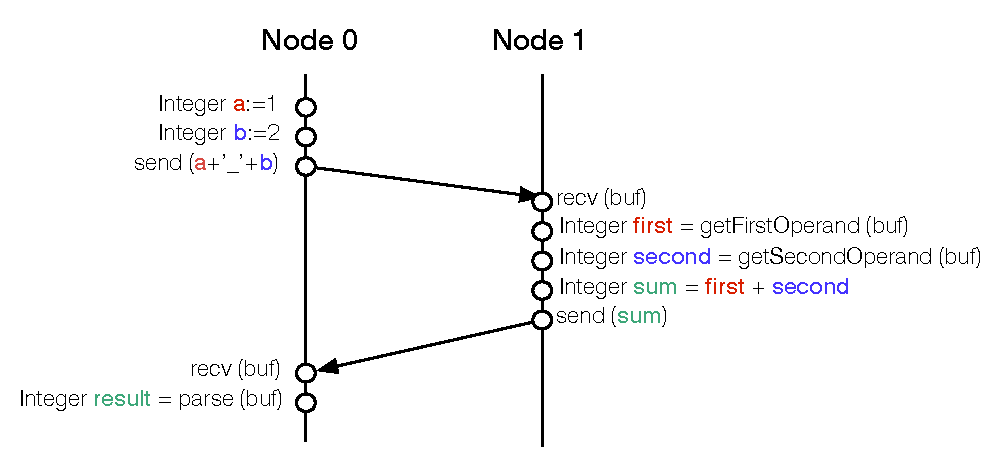
\includegraphics[width=\columnwidth]{sample_code.pdf}
  \caption{Example communication between two nodes in a distributed system}
  \label{fig:sample_code_diag}
\end{figure}

\begin{figure}
\begin{lstlisting}[caption={Sample code for Communication between 2 nodes - Node 0}, label=lst:node0]
    Integer a := 1
    Integer b := 2
    send ( a + '_' + b )
    recv (buf)
    Integer result := parse (buf)
\end{lstlisting}
\end{figure}

\begin{figure}
\begin{lstlisting}[caption={Sample code for Communication between 2 nodes - Node 1}, label=lst:node1]
    recv (buf)
    Integer first := getFirstOperand( buf )
    Integer second := getSecondOperand( buf )
    Integer sum := first + second
    send ( sum )
\end{lstlisting}
\end{figure}

As mentioned earlier, the naive approach for inferring these invariants will be to dump all
state variable values at all program points and feed them to an
invariant detector like Daikon\cite{ernst2007daikon}. But given the
number of program points and huge number of variables in a relatively
large program this approach is not scalable. Moreover, it can result in inferring incorrect invariants that are hold by accident. So we propose two main
optimizations to reduce the number of program point, variable value
combinations.

\subsection{Detecting interesting program points}

Rather than dumping state at all program points we expect the
developer to mark interesting program points using annotations. The
program state will be dumped at only these annotated points. This will
also help to narrow down the focus to points that are identified by
the developer as interesting points without wasting resources
analyzing useless program points. The annotations will be identified
by the parser at the instrumentation phase and re-written to include
statements which will write the values of variable to a file when the
program reaches that point in the runtime. Since there can be multiple points annotated in a program by a
developer, vector clocks will be used to partially order annotation
pairs in the two programs.% This will also help to invalidate
% annotations inserted at irrelevant locations by the developer.

\subsection{Data and Control Flow analysis for Go programs}

Even at interesting program points, variable space that need to be
captured is very large and also we want to filter out irrelevant invariants by only considering variables that affect each other for invariant detection phase. So only the variables that were affected by
the communication with other nodes need to be identified (distributed state variables).  To detect
these variables, some form of data and control flow analysis is required. For example using a backward flow analysis on Listing~\ref{lst:node1} we can say that \texttt{sum} variable at line 4 and line 5 is affected by the \texttt{buf} variable and receive function at line 1. Note that \texttt{sum} variable is part of distributed state of the system, since its value is affected by a receive function and affects a send function, so it is possibly affected and affects variables in other nodes of the system (here it is affected variables \texttt{a} and \texttt{b} and affects \texttt{result} in Node 0). To compute these distributed state variables, we developed a Go program slicer which we explain in the following section.

\subsubsection{Go Program Slicer}

``A program slice consists of the parts of a program that (potentially) affect the values computed at some point of interest"\cite{Tip}. For example figure \ref{Fig:backslice} illustrates an example Go program and its computed backward slice from line 11, the sliced program only contains statements that affect value of variables used at line 11 (i.e. product). To identify variables affected by the communication with other nodes we computed the forward slice from receive message functions and computed backward slice from send message functions and determined the variables assigned in these sliced statements. To compute these forward and backward slices we used the approach first proposed by Ottenstein and Ottenstein \cite{PDG}, which used Program Dependence Graph (PDG) and computed slices by checking the reachability of nodes in this graph. PDG captures both control dependency and data dependency of the program, in fact PDG is computed by combining both Data Dependence Graph and Control Dependence Graph (CDG) of a program. For example figure \ref{fig:expdg} depicts the PDG of example program of figure \ref{Fig:backslice}. Figure \ref{fig:pdg} illustrates our approach to compute PDG. First, we computed the Control Flow Graph (CFG) of the program, then from the reversed CFG we computed the post-dominance tree. The Dominance tree is computed by the algorithm proposed by Lengauer and Tarjan \cite{Dom}. In the next step we computed the CDG from post-dominance tree. To compute Data Dependence Graph, first we computed the reaching definitions by solving dataflow equations\cite{dragonbook} and then used $(Def,Use)$ pair to compute the data dependency between associated statements and form Data Dependence Graph. We combined Data and Control Dependence Graphs to compute the PDG. Having the PDG of the program we checked the reachability of nodes in PDG starting from start node to compute forward and backward slices. For example, In PDG of figure \ref{fig:expdg} thick lines are control dependence edges and thin lines are data dependence edges, starting from \texttt{send(product)} node and going backward shaded nodes are reachable, so the shaded nodes are in backward slice of \texttt{send(product)} statement.


\begin{figure}
\begin{subfigure}[b]{\linewidth}
\centering
 \begin{lstlisting}[]
	recv(n)
	i := 1
	sum := 0
	product := 1
	for i <= n {
		sum := sum + i
		product := product * i
		i := i + 1
	}
	send(sum)
	send(product)
\end{lstlisting}
        \vspace{-2mm}
                \caption{A Go Program}
        \end{subfigure}

\begin{subfigure}[b]{\linewidth}
\centering
\begin{lstlisting}[]
	recv(n)
	i := 1

	product := 1
	for i <= n {
		
		product := product * i
		i := i + 1
	}
	
	send(product) // backward slice from here
\end{lstlisting}
        \vspace{-2mm}
                \caption{Go program backward sliced at line 10}
%                \label{Fig:refactored}
        \end{subfigure}
                        \caption{Backward slice of a Go program \cite{Tip} }
                \label{Fig:backslice}
\end{figure}


\begin{figure}
  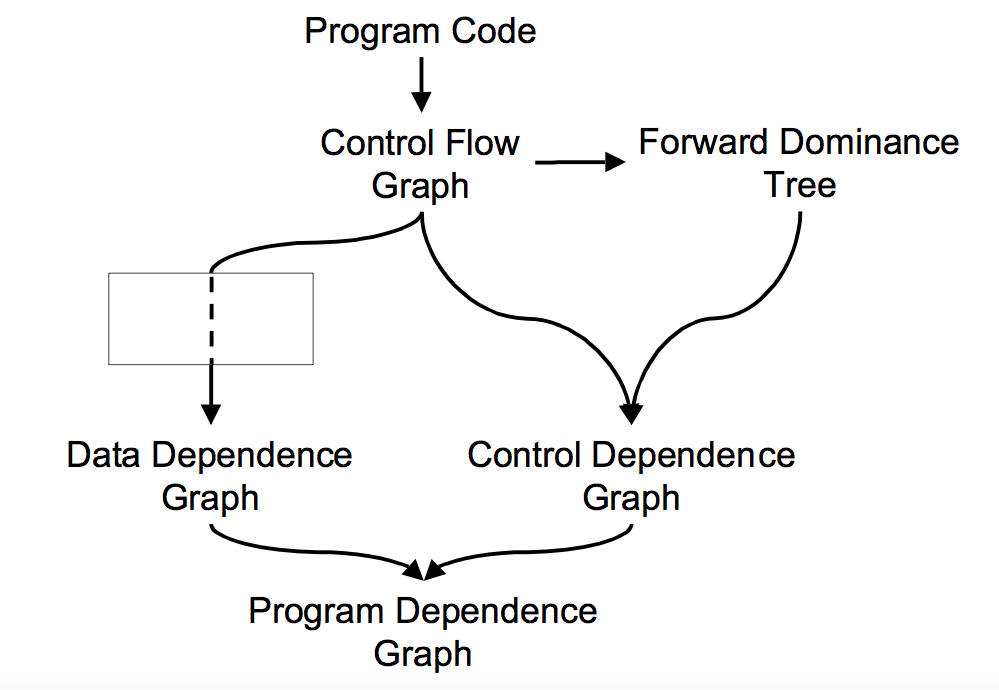
\includegraphics[width=\columnwidth,scale=0.5]{images/PDG-approach.png}
  \caption{Our approach to compute program dependence graph}
  \label{fig:pdg}
\end{figure}


\begin{figure}
  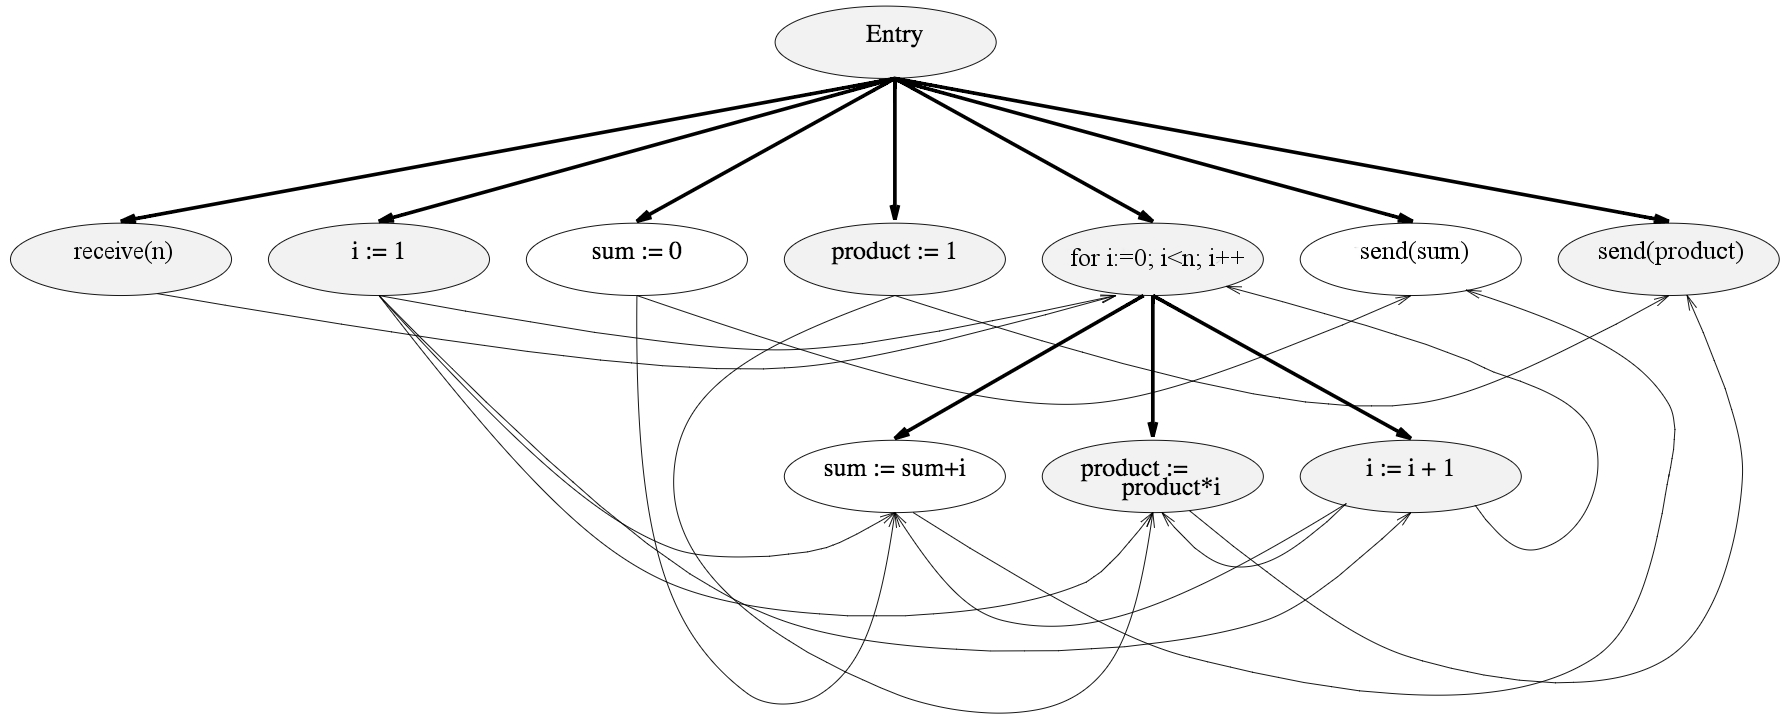
\includegraphics[width=\columnwidth,scale=0.5]{images/pdg.png}
  \caption{Program Dependence Graph of Example Program in Figure \ref{Fig:backslice}}
  \label{fig:expdg}
\end{figure}





%So we are planning to do a dynamic dataflow analysis which consists of following steps:
%\begin{itemize}
%\item Instrumenting variable declarations and assignments at the run time
%\item Collecting execution traces of each of these statements by runnning test suites
%\item Doing a forward flow analysis using the collected traces
%\end{itemize}

%This dynamic analysis approach was chosen because it gives information about the actual execution and therefore is more accurate. And also compared to using a static analysis-based approach, this approach makes it easier to handle Go language-specific constructs like channels which are used share data between goroutines. Only drawback in this approach is, it only examines the paths invoked during execution, unlike static analysis which can be used to reason about all possible execution paths and variable values. To compensate for that we are planning to use a comprehnsive test suite with good test coverage.

% This is a challenging problem in itself because Go language has
% special constructs like channels to share data between goroutines. We
% are planning to do this analysis dynamically by instrumenting variable
% declarations and assignments, and then collecting execution traces of
% each of these statements. We have chosen this approach because it
% gives information about the actual execution and therefore is more
% accurate. For this we are hoping to use static analysis libraries
% available under Go-lang tools\cite{static_golang} which provide
% support for Identifier resolution, Type information, Call graph
% navigation and Channel peers (send $\leftrightarrow$ receive)
% identification.

% Our dynamic dataflow analysis is focused on mainly providing the
% following features. Given a variable, start line and end line it will
% return a set of variables affected by that variable between start line
% and the end line.

% As the next phase of our project, using the above analysis, we hope to
% find out variables affected by receiving messages in interprocess
% communication channels like RPC and TCP/UDP sockets. We will get the
% values of these variables just before another send/receive or end of
% function whichever occurs first. We assume these set of variables at
% the send statement in both (sending and receiving) nodes taken
% together represent global state of the distributed system.

% Given two nodes which are communicating we have two such sets of
% variables representing a particular state. So we will select the
% corresponding variable pairs from send and receive of each node
% mentioned in the previous step and provide as inputs for the Daikon
% invariant detector. This will give us a set of properties that were
% true over the observed executions across 2 nodes. Overall execution
% flow of the analysis is shown in Figure~\ref{fig:go_flow}.

Overall execution flow of the analysis is illustrated in Figure~\ref{fig:go_flow} and works as follows:
\begin{itemize}
\item Developer annotates interesting program points in the Go program which will be used as states for mining invariants.
\item Program Dependence Graph is computed and based on the location of send, receive and developer annotated points, set of variables that contribute to distributed state of the system and thus should be dumped at each point is determined
\item Program is instrumented to dump selected variable values, their type and current vector clock at the annotated program points at run time
\item Based on the vector clock of each log, logs are paired to each other and combined variable values of two logs is fed to the daikon in its specific format.
%For this we are hoping to use static analysis libraries
%available under Go-lang Parse package and tools\cite{static_golang} which provide
%support for Identifier resolution, Type information, Call graph
%navigation and Channel peers (send $\leftrightarrow$ receive)
%identification.
%\item Then as the first step in the analysis phase, this instrumented program is executed using the test suites and program traces are collected.
%\item Forward flow analysis is done on the collected traces
%\item Using the results of the previous step, variables contributing to distributed state is identified.
%\item From the dumped variable values at annotated program points (after multiple executions), only the values of variables chosen in the previous step are selected.
%\item Selected variable values belonging to 2 distinct annotated program points in the 2 nodes are fed to Daikon for inferring invariants.
\end{itemize}


\begin{figure}
  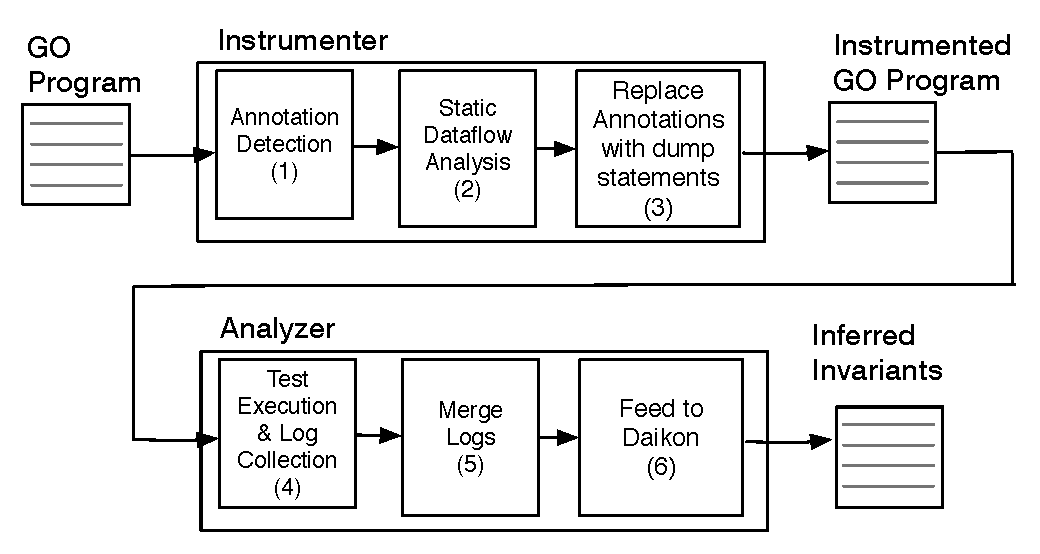
\includegraphics[width=\columnwidth]{go_flow.pdf}
  \caption{Flow of the invariant inference of Go programs}
  \label{fig:go_flow}
\end{figure}

% \section{Timeline}

% Following is the planned milestones and estimated timeline for the project completion.

% \begin{description}
%   \item[2/10:] Proposal Draft Submission
%   \item[3/3:] Proposal Submission
%   \item[3/7:] Finalizing the design, Familirization with required tools (Daikon, Go source analysis tools)
%   \item[3/14:] Implementation - Go program instrumentation to handle annotations and dumping state
%   \item[3/21:] Implementation - Dynamic Forward Analysis for Go programs
%   \item[3/28:] Implementation - Vector clocks integration and end-to-end working analysis
%   \item[4/4:] Evaluation - Inferring invariants in test programs
%   \item[4/7:] Project Presentation
%   \item[4/16:] Project Code and Report Submission
% \end{description}


\section{Implementation}

\subsection{Program Slicer}

Go program slicer is built on top of CFG and reaching definitions computed as part of Go Doctor (The Golang Refactoring Engine) project \cite{godoctor}. Also, some code snippets from Go static single-assignment (SSA) package \cite{ssa} is used to compute dominance tree from CFG. After building PDG, reachability of nodes from start node is determined via a breadth-first search on the graph.



\section{Results}
We will implement our approach in a tool in Go programming language. We plan to evaluate our tool by verifying correctness of two-phase commit and leader election protocols. Our tool should be able to infer safety property of both algorithms. In two-phase commit protocol all nodes should perform the same action (commit or abort) so our tool should infer this property. In leader election algorithm there should be only one leader (uniqueness property) and at the end of protocol execution all nodes should know ID of the leader (agreement property). It is worth mentioning that our approach is not suitable for checking the liveness properties of these algorithms.

\section{Related Work}

Yabandeh et al.\cite{yabandeh2011finding} proposed an approach to
infer almost-invariants in distributed systems. They infer the
invariants that are true in most cases and assume these invariants
only get violated due to manifestation of bugs. There are a number of
ways our approach differ from theirs: Their approach requires user to
provide a list of variables and functions that they want to consider
for inferring invariants while our approach infers distributed state
variables automatically. Moreover, they assume that an external module
generates a trace of globally consistent state system for their
algorithm while our approach extract these states through dynamic
execution of the distributed system.

Ernst et al.\cite{ernst2001dynamically} infer invariants in a
sequential program by executing the program on a collection of inputs.
This invariant detector has been released as a tool called
Daikon\cite{ernst2007daikon}. Although, we use their tool to infer
invariants, detecting invariants in a distributed system poses unique
challenges to identify distributed state and valid global states among
a larger set of variables. Ne Win et al.\cite{NeWinEGKL04} use daikon
to assist theorem provers for verifying distributed algorithms. To
demonstrate their approach, they proved the correctness of the Paxos
algorithm.

Beschastnikh et al. \cite{temporalInv} infer temporal invariants from partially ordered logs of the distributed system. By using logs of the system, they put the responsibility on developers to decide which portion of the state of the program can be used to infer invariants. Although, we require developers to specify at which points in the program invariants can be checked, we infer the portion of the state that can be checked for invariants automatically with data flow analysis.


\section{Acknowledgment}
We would like to thank Ivan Beschastnikh for his valuable insight and feedback on initial draft of this proposal.


\bibliographystyle{IEEEtran}
\bibliography{paper}





% that's all folks
\end{document}


